% class
\documentclass[a4paper,12pt,xelatex,ja=standard]{bxjsarticle}

% packages
%% mathematical notations
\usepackage{amsthm,amsmath,amssymb,amsfonts} % mathematical notations
\usepackage{bm} % bold character
\usepackage{latexsym} % more mathematical notations
\usepackage{physics} % physical notations
\usepackage{mathtools} % math tools
%% graphs
\usepackage{graphicx, xcolor} % graph
\usepackage{circuitikz} % for circuit elements
\usepackage{float} % positioning of graphs
\usepackage{siunitx} % SI units
\usepackage{tikz} % graphic elements
\usepackage{wrapfig} % must be after float package.
\usepackage{askmaps} % Karnaugh map
%% type system
\usepackage{bussproofs} % proof tree
%% code
\usepackage[ruled,vlined]{algorithm2e} % pseudo code
\usepackage{listings} % source code
\usepackage{inconsolata}
\lstset{
  basicstyle=\footnotesize,
  numbers=left,
  frame={tb}
}
\usetikzlibrary{automata, positioning}
\tikzset{
  ->,
  >={Stealth[round]},
  auto,
  every state/.style={draw}
}

% Basic information
\title{電子情報学専攻 \, 専門 \\ 平成28年 \, 解答・解説}
\author{diohabara}
\date{\today}

\begin{document}
\maketitle

\section*{第1問\ 電気・電子回路}

\section*{第2問\ 論理回路}
\subsection*{(1)}
タイムチャートは次の通り。
\begin{figure}[H]
  \centering
  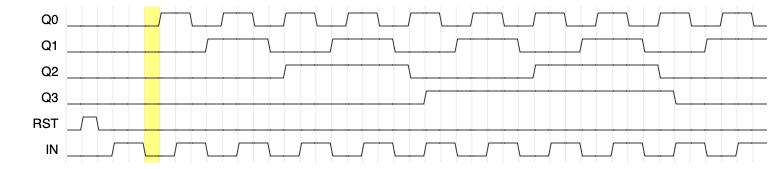
\includegraphics[width=11cm]{images/2017_timechart.png}
\end{figure}

\subsection*{(2)}
\begin{figure}[H]
  \centering
  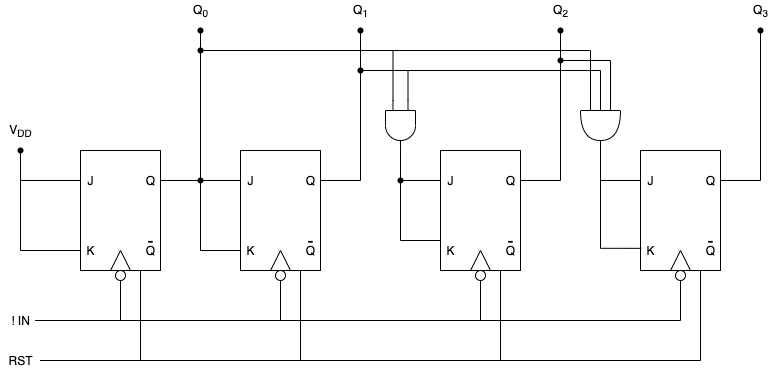
\includegraphics[width=11cm]{images/2017_synchronous_counter.png}
\end{figure}

\subsection*{(3)}
状態遷移図は以下の通り。

カルノー図は以下の通り。

\subsection*{(4)}
10進並列カウンタの回路図は以下の通り。

\subsection*{(5)}
求める(2)で設計したカウンタをアップダウンカウンタに改変したものは次の通り。

\section*{第3問\ アルゴリズムとデータ構造}
\subsection*{(1)}
求めるリストLの値の推移は以下の通り。
\begin{table}[]
  \begin{tabular}{|l|l|l|}
  \hline
  \textit{i} & A[i] & L            \\ \hline \hline
  0          & 11   & {11}         \\ \hline
  1          & 10   & {}           \\ \hline
  2          & 11   & {11}         \\ \hline
  3          & 11   & {11, 11}     \\ \hline
  4          & 7    & {11}         \\ \hline
  5          & 11   & {11, 11}     \\ \hline
  6          & 11   & {11, 11, 11} \\ \hline
  7          & 3    & {11, 11}     \\ \hline
  8          & 8    & {11}         \\ \hline
  \end{tabular}
\end{table}

\subsection*{(2)}
$i$番目の要素を処理した後のLの要素の種類数は0または1である。\\
$i+1$番目の要素を処理した後も種類数が0または1であるから帰納法よりLに含まれる要素の種類数は高々1つである。

\subsection*{(3)}
Lに含まれる要素が高々1つであることは(2)で示した。よって、全ての要素を処理した後のLに$u_{MAJORITY}$が含まれることを証明すれば良い。\\
\begin{proof}[証明]
  \[
    \text{count} \coloneqq \text{(Lに含まれている$u_{MAJORITY}$の個数)} - \text{(Lに含まれている$u_{MAJORITY}$以外の要素の個数)}
  \]
  として、処理が終わったときに$0 < count$であることを示す。はじめ、Lは空であるので$count = 0$。A[i]に対して処理を行うとき\\
  \subsubsection*{(i) $A[i] = u_{MAJORITY}$の場合}
  \begin{itemize}
    \item Lに$u_{MAJORITY}$を追加する
    \item Lから$u_{MAJORITY}$以外の要素を1つ取り除く
  \end{itemize}
  のどちらかである。よってcountは1大きくなる
  \subsubsection*{(ii)$A[i] \neq u_{MAJORITY}$の場合}
  \begin{itemize}
    \item LにA[i]を追加する
    \item Lから$u_{MAJORITY}$を1つ取り除く
    \item Lから$u_{MAJORITY}$以外の要素を1つ取り除く
  \end{itemize}
  のいずれかである。
  (i)(ii)からすべての処理が終わったとき
  \[
    \text{(Aに含まれている$u_{MAJORITY}$の個数)} - \text{(Aに含まれている$u_{MAJORITY}$以外の要素の個数)} \leq count
  \]
  であるので、$u_{MAJORITY}$が過半数であることから$0 < count$となる。したがって、過半数を占めるユーザ$u_{MAJORITY}$が存在するとき$u_{MAJORITY}$はLに含まれる唯一のユーザである。
\end{proof}

\subsection*{(4)}
\begin{lstlisting}[language=Python]
u = -1 # Lに含まれるユーザ
counter = 0 # Lに含まれるユーザ数
while True:
    v = read_log()
    if v == -1:
        break
    if counter == 0:
        u = v
        counter = 1
    else:
        if v == u:
            counter += 1
        else:
            counter -= 1
while 0 < counter:
    print(u)
    counter -= 1
\end{lstlisting}

\section*{第4問\ 情報通信}

\section*{第5問\ 情報理論}
\subsection*{(1)}
出力のデータを表にすると以下の通り。

\begin{table}[H]
  \centering
  \begin{tabular}{|l|l|l|l|l|l|}
  \hline
  1 & 2 & 3 & 4 & 5 & 合計 \\ \hline
  1 & 3 & 5 & 5 & 2 & 16 \\ \hline
  \end{tabular}
\end{table}

よって、ランダム系列とみなしたときのエントロピーは
\begin{equation*}
  \begin{split}
    H
      &= - (\frac{1}{16} \log (\frac{1}{16}) + 2 \cdot \frac{3}{16}\log (\frac{3}{16}) + 2 \cdot \frac{5}{16} \log (\frac{5}{16}))\\
      &= \log 16 - \frac{1}{16} (3 \log 3 + 10 \log 5 + 2 \log 2) \\
      &= 4 - \frac{1}{16}(3 \cdot 1.6 + 10 \cdot 2.3 + 2) = 2.1375 \approx 2.14 \text{[bit]}
  \end{split}
\end{equation*}

\subsection*{(2)}
ハフマン符号化する。以下の通り。

\begin{figure}[H]
  \centering
  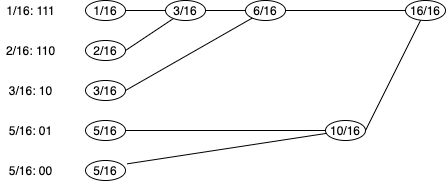
\includegraphics[width=11cm]{images/2017_huffman_tree.png}
\end{figure}

このとき、平均符号長は以下のように2.2bitより小さくなる。
\[
  2 \cdot 3 \cdot \frac{5}{16} + 3 \cdot \left(\frac{2}{16} + \frac{1}{16}\right)= \frac{35}{16} = 2.1875 (< 2.2) \text{[bit]}
\]

\subsection*{(3)}
条件として$\alpha, \beta \in \mathbb{Z}$かつ$\alpha + \beta = 1$かつ$b_n$のエントロピーが1.0。
$\alpha + \beta = 1$の条件を使うため、$a_{n-1} = a_{n-2}$のパターンについて見ていく。

\begin{itemize}
  \item $n = 5$のとき、$a_n = 3, a_{n-1} = a_{n-2} = 4$となることから$b_n = -1$
  \item $n = 7$のとき、$a_n = 4, a_{n-1} = a_{n-2} = 3$となることから$b_n = 1$
\end{itemize}

これより、$b_n = \pm 1$となることが必要条件。\\

次に$(\alpha, \beta)$の組に注目する。\\

\begin{itemize}
  \item $n = 2$のとき、$(a_n, a_{n-1}, a_{n_2}) = (3, 5, 2)$となるが、$\alpha \leq 1$のとき、$a_2 \leq 4$となり不適当
  \item $n = 3$のとき、$(a_n, a_{n-1}, a_{n_2}) = (4, 3, 5)$となるが、$\beta \leq 2$のとき、$a_3 \leq 6$となり不適当
\end{itemize}

したがって、$(\alpha, \beta) = (0, 1)$が候補に残る。\\

最後に表よりすべての$n \leq 2$に対して$a_{n} = a_{n-2} \pm 1$が成り立っているので、求める出現確率は$(\alpha, \beta) = (0, 1)$

\subsection*{(4)}
$a_0, a_1$で必要な符号長は$5 \text{[bit]}$。それ以降は$b_n$の情報だけで十分なので、$b_n$が$1$なのか$-1$なのかの情報を$1 \text{[bit]}$ずつ送れば伝達は可能。\\
したがって、求める符号長は$5 + 14 = 19\text{[bit]}$。

\subsection*{(5)}
\begin{enumerate}
  \item $X_1, \dots, X_n$が互いに独立でない場合、$n$個を合わせたときに得られる情報量は単純な足し合わせにはならない。したがって、$X_1, \dots, X_n$の中に相関がある場合。情報量が減ってしまうから。
  \item $X_1, \dots, X_n$を受け取って$Y$から出力する際に、情報が抜け落ちてしまう場合。情報量が落ちてしまうから。
  \item ビット誤りや$Y$の内部状態によって出力が変化する場合。$X_1, \dots, X_n$とは関係のない情報を添加していることになるので情報量が増える要因となるから。
\end{enumerate}

\end{document}
